\chapter{Background Theory}

To understand the rest of this thesis, some basic knowledge about low-power design, accelerometers in general and microelectromechanical systems (MEMS) are required. This chapter presents an overview of these topics. The presented theory in this chapter is regarded as well-established, and is covered in several books and papers.

It is assumed that the reader has a basic understanding of embedded systems, as well as some knowledge of basic physical principles. 

\section{Low Power Design}

[Maybe include something about low power design in general]

\cite{sarpeshkar12}

\subsection{Power In CMOS}
\label{sec:cmos_power}

The power consumption in CMOS circuitry can in general be divided into two different domains, static and dynamic power consumption. Static power consumption comes from leakage current in the transistor, which is a result of reverse-bias leakage between diffused regions and the
substrate in the transistor \cite{static_dynamic_power}. The static power consumption ($P_{static}$) is given by the product of the static current ($I_{static}$) and the supply voltage ($V_{ss}$), as seen in Equation \ref{eq:p_static}. 

\begin{equation}
P_{static} = I_{static} \cdot V_{ss}
\label{eq:p_static}
\end{equation}

Dynamic power consumption is result of switching the logic state of the transistor, which is given by the sum of the transient- and capacitive-load power consumption. The transient power ($P_{transient}$) consumption is from the current that flows through the transistor when the the transistor is switching logic state, while the capacitive-load power ($P_{capacitive}$) is from the additional current consumed in charging external load capacitance ($C_{L}$) \cite{cmos_power_consumption}. The dynamic power consumption is dependent on the frequency ($f$) as well as the number of transistors that are switching ($N$). The dynamic power consumption is also proportional to the supply voltage ($V_{ss}$) squared. This relationship can be seen in Equation \ref{eq:p_dynamic}.

\begin{equation}
P_{dynamic} = P_{transient} + P_{capacitive} = (C_L + C) \cdot V_{ss}^{2} \cdot f \cdot N^3
\label{eq:p_dynamic}
\end{equation}

From Equation \ref{eq:p_dynamic} one can see that the dynamic power consumption is proportional to the frequency. This means that a higher performance generally leads to a higher power consumption. Another important aspect to note, is that the supply voltage is present both in the static and dynamic power consumption of CMOS circuits. Reducing the voltage is therefore very important when it comes to reducing the overall power consumption in a CMOS circuit.

\subsection{Power Saving Peripherals}

\subsubsection{DMAC - Direct Memory Access Controller}

Most of today's modern microcontrollers feature a Direct Memory Access Controller (DMAC). A DMAC is simply put a peripheral device that can be configured to move data from one location in memory to another. Usually, a DMAC is also able to transfer data from and to peripherals as well. DMA is primarily used as a technique to offload the CPU for large data transfers. This enables the CPU to do other work while the DMAC is moving data, thereby increasing overall system performance. However, a DMAC can also be used to improve power efficiency in a system. By combining a DMAC and an event system one is able to do certain operations without any CPU intervention. This is very beneficial, since both the event system and DMAC uses much less power than the CPU core. This scheme is often utilized as a power saving technique in modern embedded systems \cite{ball03}.  

\subsubsection{Event system}

Most modern microcontrollers have a variant of a so called event system. An event system enables different peripherals in the microcontroller to interact autonomously with each other by using tasks and events. By using such a system one is able to let peripherals communicate with each other without involving the CPU, and thereby saving power.

\subsubsection{Clock Gating}

A clock gating scheme is all about turning off the clock for the unused domains of the chip. Clock gating effectively removes the dynamic power consumption from the gated domain, which can be seen from Equation \ref{eq:p_dynamic}. The static power consumption is however still present, as voltage is still applied to the gated domain. Clock gating can for example be very beneficial for volatile memory (such as RAM), as the user can reduce power consumption while still maintaining data in memory.

\subsubsection{Power Gating}

Power gating is about completely turning off the voltage to unused blocks of the system, thereby removing both static and dynamic power consumption. Modern microcontrollers often have the ability to power gate RAM blocks, giving the user the option to trade power for RAM or vice versa. It is also common to power gate peripherals that are not used for the application.

\subsection{Energy Harvesting}

[still don't know where to put this section]

A battery will always run out of power, no matter how little current the system draws. So to be able to make a system that can continue indefinitely, one need to be able to have an infinite power source. Unfortunately, this does not exist. There is however a lot of research going into developing solutions that can turn energy from our surroundings into electrical energy. The principal is called energy harvesting, and it is truly a term that goes hand in hand with the IoT movement. Energy can be harvested from vibrations, sunlight, heat and a lot of other sources. A product that can implement one or more of these energy harvesting techniques has the potential to run indefinitely. Energy harvesting is something that has existed for a long time, but it is only with today's ultra low power components that it is actually possible to use this energy to power our devices.

\section{Acceleration}

Acceleration is defined as the rate of change in velocity with respect to time. It is given by a vector with both magnitude and direction relative to a reference frame. The SI units are length divided by time squared \cite{elert98}.

\section{Accelerometers - Working Principle} \label{sec:accel_working_principle}

The working principle of an accelerometer can be viewed as a simple mechanical system, as illustrated in Figure \ref{fig:accel_working_principle}. A proof mass $m$ is connected to a frame by a flexible spring $k$. When an acceleration is imposed along the x-axis, the proof mass will begin to move. Due to Newton's law of inertia, the motion of the proof mass will lag the frame motion. This will cause an oscillation of the proof mass inside the frame. From this oscillation alone, it is possible to get the acceleration. However, to prevent excessive oscillation, the mass vibrations are usually damped by introducing a dampening material (such as gas or liquid) inside the package. This is represented by a dashpot $\gamma$ in Figure \ref{fig:accel_working_principle}.

\begin{figure}[h]
\centering
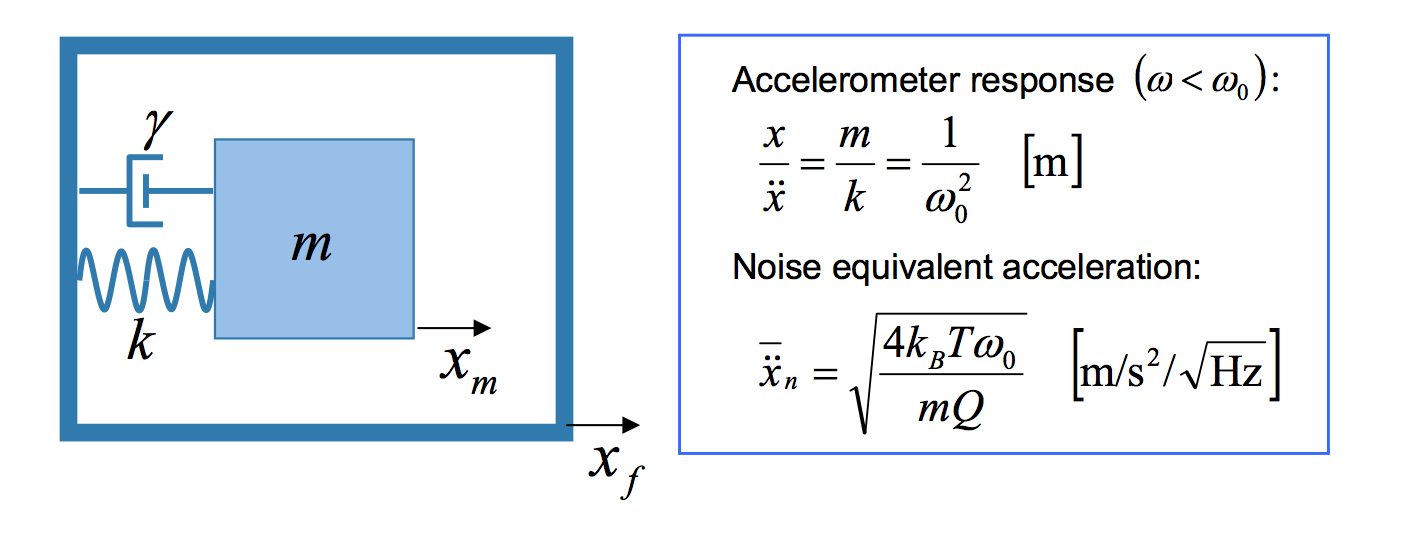
\includegraphics[scale=0.5]{fig/accelerometer_working_principle.png}
\caption{Working principle of an accelerometer \cite[~p.34]{kaajakari09}}
\label{fig:accel_working_principle}
\end{figure}

\subsubsection{Mechanical noise in accelerometers}
\label{sec:mechanical_noise}
The mechanical noise in an accelerometer is usually specified by the power spectral density (PSD), given by Equation \ref{eq:noise_spectral_density}. If we analyse this equation more closely, we see that the thermal noise energy $k_b T$ is a constant irrespective of the system size \cite[~p.13]{kaajakari09}. This means that the thermal noise induced in mechanical vibrations sets the lower limit for the smallest, measurable acceleration \cite[~p.41]{kaajakari09}. One can also see from Equation \ref{eq:noise_spectral_density} that increasing the mass $m$ and reducing the resonant frequency $\omega_0$ reduces the overall noise. The $Q$ factor, or quality factor, is a dimensionless parameter that describes how under-damped an oscillator or resonator is \cite[~p.216]{harlow04}. Again, we can see from Equation \ref{eq:noise_spectral_density} that increasing the Q factor helps reducing the overall noise.

\begin{equation}
\bar{\ddot{X_n}} = \sqrt{\frac{4 k_b T \omega_0}{mQ}}
\label{eq:noise_spectral_density}
\end{equation}

\section{Microelectromechanical Systems (MEMS)}

Microelectromechanical Systems (MEMS) are embedded systems involving one or many micromachined components or structures\cite[p.~3]{maluf04}. The technique is used for a vast number of applications ranging from accelerometers and gyroscopes to fluid nozzles on a inkjet printer.

\subsection{MEMS Accelerometers}

The basic working principles of an accelerometer, described in section \ref{sec:accel_working_principle}, also applies for all types of MEMS accelerometers. The different MEMS accelerometers do however differ in the way that they sense the displacement of the inertial mass. One of the most common methods involve sensing the change in capacitance when the inertial mass is displaced, then converting it into an amplified output voltage. Another method involves sensing the internal stress in the spring by using piezoresistors. One also see solutions were the spring is replaced with a piezoelectric element, providing a voltage in direct proportion to the displacement itself.

The first micromachined accelerometer was demonstrated at Stanford University in 1979. However, it took nearly 15 years for the technology to become accepted into mainstream products \cite[p.~8]{maluf04}. The automotive industry has undoubtedly been a big contributor for the technology, as accelerometers has an apparent application in detecting crashes for airbag deployment systems. MEMS accelerometers has in recent years also found its way into other applications, such as smart phones, quad-copters and game controllers. 

\subsection{MEMS Processing Techniques}

\subsubsection{Surface Micromachining}

Surface micromachining is based on patterning deposited thin film materials on top of a substrate wafer \cite[p.~5]{kaajakari09}. The production technique first appeared in the 1980s, and was primarily used as a low cost alternative to accelerometers for the automotive industry \cite[p.~101]{maluf04}. However, recent improvements in the production technique has made it possible to use the technique for other sensors such as pressure sensors, gyroscopes and microphones. 

The surface micromachining process bear a close resemblance to the traditional integrated circuit (IC) manufacturing process, which is also based on processing thin films on a silicon wafer. In fact, the processes are so close that a retired IC manufacturing plant often are converted into a MEMS fabrication plant, as MEMS does not require the latest in fabrication technology \cite[p.~4]{kaajakari09}. The similarities between IC manufacturing and surface micromachined MEMS has several advantages. It is for instance relatively easy to integrate MEMS architectures together with IC to make a single-chip solution, which often leads to better performance and reduced packing-cost. 

\subsubsection{Surface Micromachined Accelerometers}

Surface micromachined accelerometers incorporates a comb-like structure, as depicted in Figure \ref{fig:surface_micromachined}. The primary axis is located in the plane of the die, and is often referred to as an x-axis or y-axis. Two sets of electrodes are anchored down in the substrate. These two electrodes are interlaced with a third set connected to the inertial mass. This mass is being suspended over the surface by means of two long beams, acting as a suspension spring. Thereby, it is free to move about as acceleration is applied along the primary axis. When the inertial mass is displaced due to an acceleration, it is causing the capacitance to change between the fingers of the comb-like structure. The change in capacitance is typically very small, in the order of 100 $\si{\femto\farad}$ \cite[p.~101]{maluf04}. To mitigate this problem, several sensing fingers are often combined in parallel to increase the overall capacitance.

\begin{figure}[h]
\centering
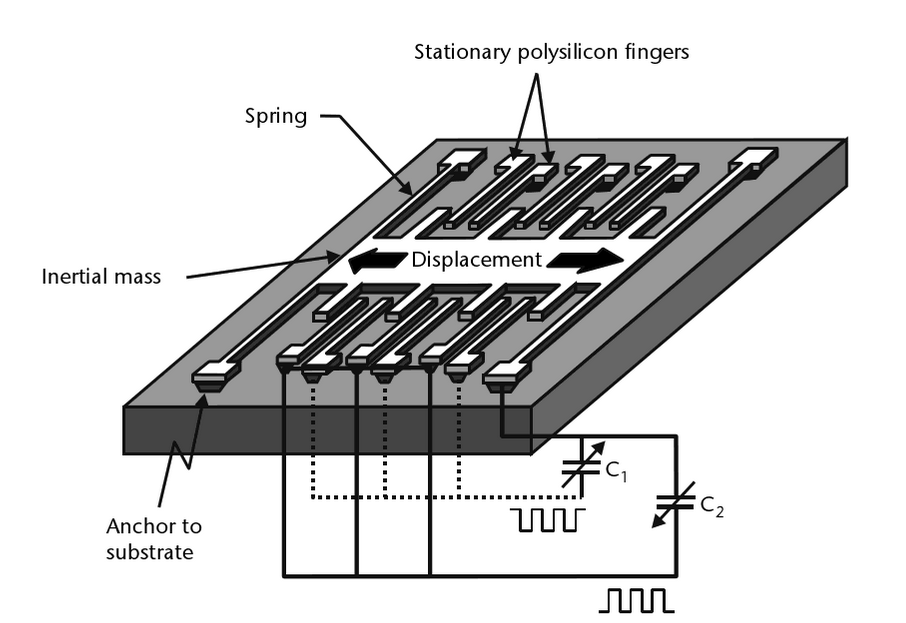
\includegraphics[scale=0.3]{fig/surface_micromachined.png}
\caption{Illustration of surface micromachined accelerometer from Analog Devices ADXL family \cite[p.~101]{maluf04}}.
\label{fig:surface_micromachined}
\end{figure}

\subsubsection{Bulk Micromachining}

Bulk micromachining defines structures by selectively etching the substrate \cite[p.~7]{kaajakari09}. This makes it possible to etch much thicker structures when being compared to the surface micromachining process. A typical thickness of bulk micromachined structure is between 500$\si{\micro\meter}$-700$\si{\micro\meter}$, which is about a 100 times the typical thickness of a surface micromachined structure \cite[p.~7]{kaajakari09}. A thicker structure means more mass, which is very beneficial in terms of reducing the noise, which can be seen from Equation \ref{eq:noise_spectral_density}. Bulk micromachined structures can also be made of a single-crystal silicon as opposed to thin film materials in surface micromachined structures. This is very beneficial, since these materials are very predictable and stable. Bulk micromachined accelerometers either use piezoresistive elements or capacative sensing to detect the displacement of the inertial mass.

Pressure sensors and accelerometers were the first commercial products that utilized the bulk micromachining technique. These devices have been very successful, as 90\% of all sold pressure sensors utilize this technique \cite[p.~7]{kaajakari09}. The production process is however more complicated and expensive than surface micromachining, and has therefore lost market shares in the recent years.

\subsubsection{Piezoresistive Bulk Micromachining Accelerometer}

Electrical resistance changes due to mechanical stress. This effect occurs in all materials and it is called the piezoresistive effect \cite[p.~73]{kaajakari09}. For an accelerometer of this type, piezoresistive springs are used to sense the displacement of the inertial mass. In general, the sensing technique offers two advantages. The resistance measurement circuitry is very simple to implement compared to that of capacitive sensors. The second is that piezoresistors are inherently shielded structures, so no hermetic packaging is required. However, piezoresistive sensing suffers from noise, as the elements themselves has a large temperature dependency, and they also consumes a significant amount of power. Because of this, sensors with this sensing technique has lost market share to capacitive sensors.

\begin{figure}[h]
\centering
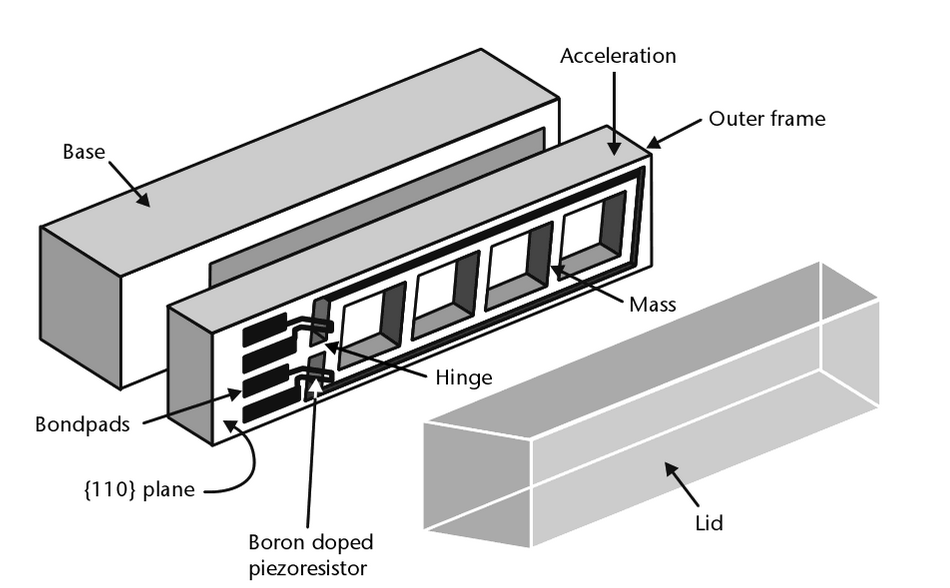
\includegraphics[scale=0.3]{fig/piezoresistive.png}
\caption{Illustration of piezoresistive accelerometer from Endevco Corp. \cite[p.~98]{maluf04}}
\label{fig:piezoresistive_accel}
\end{figure}

\subsubsection{Capacitive Bulk Micromachining Accelerometer}

A capacitive bulk micromachined accelerometer measures the differential change in capacitance when the inertial mass is displaced. Capacitive sensors provides an excellent noise performance and low power consumption \cite[p.~91]{kaajakari09}. One of the main challenges with capacitive sensors is to accurately measure the change in capacitance, as these changes themselves are extremely small. 

\begin{figure}[h]
\centering
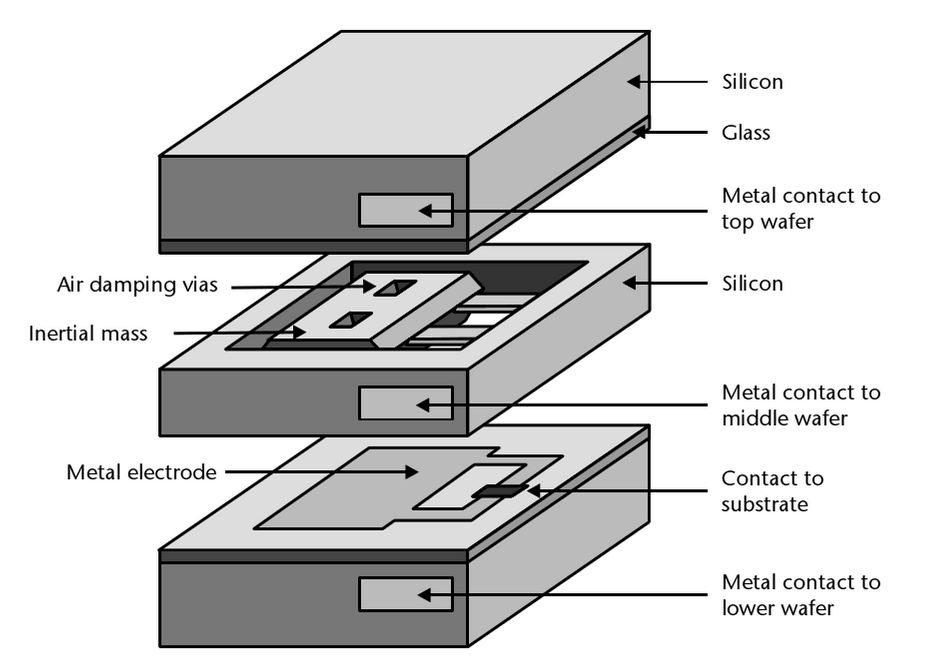
\includegraphics[scale=0.25]{fig/bulk_micromachined.png}
\caption{Illustration of capacative bulk micromachined accelerometer. \cite[p.~100]{maluf04}}
\label{fig:bulk_micromachined}
\end{figure}

\subsection{Integrating MEMS and ICs}

Most MEMS based sensors must be bonded together with an IC for integration in larger electronic systems. The MEMS element itself is just a transducer, converting some physical parameter (motion, sound, pressure) into an electrical signal. Data converters, amplifiers and signal conditioning is required to be able to make use of the signal from the transducer, which requires additional logic on an IC. A typical functional block diagram of a MEMS accelerometer can be viewed in Figure \ref{fig:ADXL362_functional}. 

\begin{figure}[h]
\centering
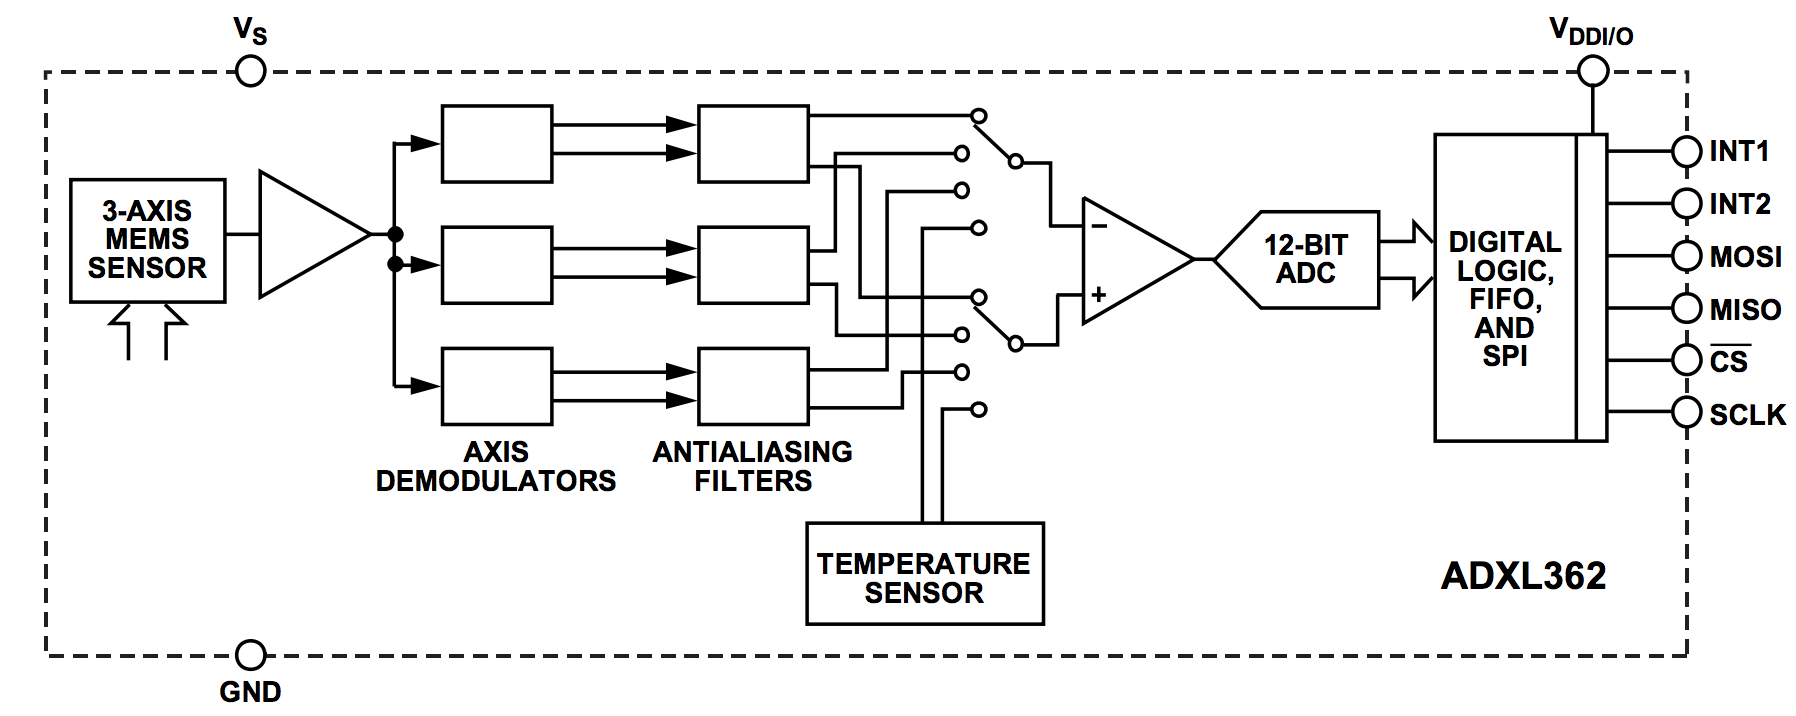
\includegraphics[scale=0.5]{fig/ADXL362_functional_block.png}
\caption{Functional block diagram of ADXL362 from Analog Devices.}
\label{fig:ADXL362_functional}
\end{figure}

MEMS and ICs can be integrated together in two separate fashions. The most common approach is to manufacture MEMS and ICs on separate substrates using their dedicated production processes respectively, and then bond them together in the final system. This approach is typically referred to as a multi-chip solution or a system-in-package (SiP), depending on whether the chips are stacked horizontally or vertically. In the other integration approach, MEMS and ICs are manufactured on the same substrate, using consecutive or interlaced processing schemes. This approach is often referred to a system-on-chip (SoC) solution \cite{fischer15}. 

\subsection{MEMS Accelerometer Parameters}

This section gives an overview, as well as an explanation, of the most common characteristics one should look for when selecting an accelerometer.

\subsubsection{Accelerometer Interface}

Primarily one differentiates between two interface types when it comes to accelerometers, analog and digital. Analog accelerometers have an output that is a continuous voltage proportional to the acceleration. An analog accelerometer is therefore best suited for a completely analog circuit. An analog to digital converter (ADC) is a required peripheral for a microcontroller to make use of such a sensor in a digital system.

Digital accelerometers typically use a serial communication interface like SPI or I2C for data transfer. They are therefore much better suited for a digital circuit, as most of today's microcontrollers usually features one or both of these serial interfaces.

From a power perspective, it is worth noting that SPI is a more efficient communication interface than I2C. This is because SPI is full-duplex and generally operates at a higher clock frequency than I2C, which means that more data can be transmitted in less time. 

\subsubsection{Number of axes}
MEMS Accelerometers are able to measure acceleration along either one, two or three axes (x,y and z). Two axes (x and y) are usually sufficient for most applications, and are therefore the most common type. 3-axis accelerometers are however becoming more and more popular. Mainly because three axes are very useful for applications such as quad-copters, smart phones and game controllers.

\subsubsection{Measurement range}
Measurement range, sometimes called swing level, is defined as the level of acceleration that is supported by the sensor’s output signal specifications \cite{analog_accel_guide}. This level is listed as a number $n$ times the earth’s gravity (i.e. $\pm$1g , $\pm$2g etc.). This number is an upper limit for the accurate measurement range of the part. For example, if the part is rated with a measurement range of $\pm$3g, it means that the part can measure the acceleration accurately up to an acceleration of $\pm$3g.  If the part is accelerated above this limit, the output might rail or be distorted at the output.

\subsubsection{Sensitivity}
The sensitivity is defined as the sensor's ratio of change in mechanical input to change in electrical output. Ideally, the ratio between the acceleration and the sensor output should be linear. In practice, all MEMS accelerometers suffers from non-linearity due to mechanical stresses and circuit temperature coefficients  \cite{analog_accel_guide}. For digital accelerometers, the sensitivity is usually specified at a specific voltage as units of mg/LSB. For example, if an accelerometer has a rating of 1mg/LSB, it means that when the lowest order bit in the output changes, the acceleration has changed by 0.001 g's (1mg).

\subsubsection{Bandwidth}

The output data rate (ODR) defines the data sample rate for digital accelerometers. The bandwidth (BW) is defined as the highest frequency signal that can be sampled without any aliasing by the specified ODR. As specified by the Nyquist criterion, the bandwidth is half the output data rate \cite{analog_accel_guide}, as seen in Equation \ref{eq:bw}. 

\begin{equation}
BW = \frac{ODR}{2}
\label{eq:bw}
\end{equation}

\subsubsection{Noise}

The noise in a MEMS accelerometer is either from mechanical noise in the MEMS element, as described in Section \ref{sec:mechanical_noise}, or as electronic noise in the IC itself. The overall noise in the system is usually given by the power spectral density (PSD) in the accelerometer datasheet, usually in the units of $\si{\micro}$g per square root Hz. The PSD captures the frequency content of a stochastic process (noise) and describes how the power is distributed across different frequencies. The noise in an accelerometer is predominantly considered to be Gaussian white noise, and is thereby a constant value across all frequencies \cite{freescale_accel_guide}. The relationship between the PSD and the root-mean-square (RMS) noise is given by Equation \ref{eq:rms_noise}, and can be simplified to \ref{eq:rms_psd_bw}.

\begin{equation}
N^{2}_{rms}=\int_0^{BW}{PSD(f)df}
\label{eq:rms_noise}
\end{equation}

\begin{equation}
N_{rms}=\sqrt{PSD \cdot BW}
\label{eq:rms_psd_bw}
\end{equation}

The PSD noise value that is listed in the component datasheets is actually the square root PSD from the derivation in Equation \ref{eq:rms_psd_bw}, which in turn gives us Equation \ref{eq:rms_psd_bw_2}.

\begin{equation}
N_{rms}=PSD_{datasheet} \cdot \sqrt{BW}
\label{eq:rms_psd_bw_2}
\end{equation}

\subsubsection{Digital Resolution}

An accelerometers digital resolution is normally specified as the number of bits in the ADC. The devices that are available today typically range between 12 and 16-bits. However, this number might sometimes be misleading. Every MEMS accelerometer suffers from system noise to a certain extent, which in turn will limit the number of effective bits in the ADC \cite[~p.3]{freescale_accel_terminology}. In other words, it does not help to have a 16-bit ADC if four of the lower bits are full of noise. The number of effective bits (ENOB) is possible to calculate if the system noise is specified in the datasheet. One first need to calculate the system noise for a specific measurement range and bandwidth. This can be done by using Equation \ref{eq:system_noise} together with Equation \ref{eq:rms_psd_bw_2}. A measurement range of $\pm$2g (4g in total) is assumed in Equation \ref{eq:system_noise}. By combining Equation \ref{eq:effective_bits} with Equation \ref{eq:system_noise} one is able to calculate the number of effective bits. 

\begin{equation}
SND(db) = 20\log{\frac{\frac{4g}{2\sqrt{2}}}{N_{rms}}}
\label{eq:system_noise}
\end{equation}

\begin{equation}
ENOB = \frac{SND(db)-1.76}{6.02}
\label{eq:effective_bits}
\end{equation}